\subsection{Game Engine}
Le GE sono framework utilizzati per supportare la progettazione e lo sviluppo di giochi. Il termine "Game Engine" nacque a metà degli anni '90 in riferimento a giochi sparatutto in prima persona (FPS) come il popolare "Doom" progettato con una separazione ragionevolmente ben definita tra i suoi componenti software principali (come il sistema di rendering grafico tridimensionale, il sistema di rilevamento delle collisioni o il sistema audio) e le risorse artistiche, i mondi di gioco e le regole di gioco che comprendevano l'esperienza di gioco del giocatore.

\medskip

La maggior parte delle GE sono realizzate con cura e messe a punto per eseguire un gioco particolare su una particolare piattaforma hardware.
L'avvento di hardware per computer sempre più veloce e schede grafiche specializzate, insieme a algoritmi di rendering e strutture di dati sempre più efficienti, sta cominciando ad ammorbidire le differenze tra i motori grafici di diversi generi. È ora possibile utilizzare un motore sparatutto in prima persona per creare un gioco di strategia, ad esempio. Tuttavia, esiste ancora il compromesso tra generalità e ottimizzazione. Un gioco può sempre essere reso più impressionante perfezionando il motore in base ai requisiti e ai vincoli specifici di una determinata piattaforma di gioco e/o hardware \cite{ge-architecture}.

\begin{figure}[H]
\centering
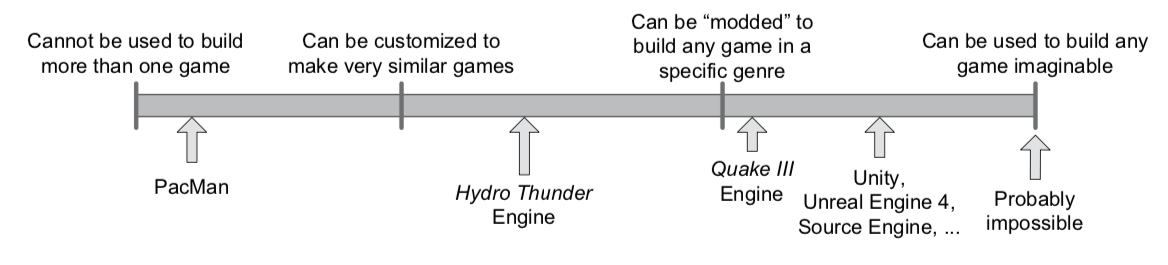
\includegraphics[width=\textwidth]{figures/Game_Engine_Reusability.png}
\caption{Game Engine reusability gamut \cite{ge-architecture}}
\end{figure}
\medskip

Le GE moderne sono strutture general-purpose multipiattaforma orientate verso ogni aspetto della progettazione e dello sviluppo del gioco, come il rendering 2D/3D delle scene di gioco, i motori fisici per la dinamica ambientale (movimenti, dinamica delle particelle, rilevamento delle collisioni, prevenzione degli ostacoli, ecc.), suoni, script comportamentali, intelligenza artificiale dei personaggi e molto altro.

\medskip

Come esempio significativo che rappresenta la gamma di piattaforme disponibili, nella sezione \ref{unity} verrà esaminata una delle più popolari GE - Unity \cite{unity} - con l'obiettivo di:
\begin{itemize}
    \item rilevare quelle astrazioni e quei meccanismi che hanno più probabilità di avere una controparte nel MAS, o almeno quelli che sembrano fornire un supporto nel riformulare le astrazioni mancanti del MAS
    \item evidenziare le opportunità per colmare le lacune concettuali / tecniche che ostacolano l'integrazione dei due mondi
\end{itemize}
